\documentclass[a4paper,12pt,english,cph,openright]{aau}

% ============================================================================
% PACKAGES
% ============================================================================
\usepackage[utf8]{inputenc}
\usepackage[english]{babel}
\usepackage[T1]{fontenc}

% MODERN FONT - Palatino-style serif for elegant readability
\usepackage{palatino}
\usepackage{mathpazo}

% Margins - COMPACT LAYOUT
\usepackage[left=2.5cm, right=2.5cm, top=2.5cm, bottom=2.5cm]{geometry}

% Line spacing - SINGLE SPACED
\usepackage{setspace}
\singlespacing

% Graphics and figures
\usepackage{graphicx}
\usepackage{wrapfig}
\usepackage{subfig}
\usepackage{float}
\usepackage{tikz}
\usetikzlibrary{positioning,shapes,arrows,calc}

% Tables - MINIMAL STYLE
\usepackage{tabularx}
\usepackage{booktabs}
\usepackage{multirow}
\usepackage{colortbl}
\setlength{\heavyrulewidth}{1.2pt}
\setlength{\lightrulewidth}{0.5pt}

% Lists - MINIMAL STYLE WITH DASHES
\usepackage{enumitem}
\usepackage{paralist}
\setlist[itemize]{label=\textendash, itemsep=2pt, leftmargin=1.5em}
\setlist[enumerate]{itemsep=2pt}

% Math
\usepackage{amsmath}
\usepackage{amssymb}

% Links and references - SUBTLE COLORED LINKS
\usepackage{hyperref}
\hypersetup{
    colorlinks=true,
    linkcolor=aaublue,
    filecolor=aaublue,
    urlcolor=aaulight,
    citecolor=aaublue,
    pdftitle={Agile Software Engineering - Exam Assignment},
    pdfauthor={Your Name},
    bookmarks=true,
    bookmarksnumbered=true,
    pdfpagemode=UseOutlines,
}

% Bibliography with BibLaTeX - AUTHOR-YEAR STYLE
\usepackage[style=authoryear,backend=biber,sorting=nyt,maxcitenames=2]{biblatex}
\addbibresource{references.bib}

% Table of contents depth
\setcounter{tocdepth}{2}
\setcounter{secnumdepth}{3}

% Headers and footers - MINIMAL EDITORIAL STYLE
\usepackage{fancyhdr}
\pagestyle{fancy}
\fancyhf{}
\fancyhead[R]{\small\textit{\nouppercase{\leftmark}}}
\fancyfoot[C]{\small\thepage}
\renewcommand{\headrulewidth}{0pt}
\renewcommand{\footrulewidth}{0pt}

% First page of chapters - no header
\fancypagestyle{plain}{
  \fancyhf{}
  \fancyfoot[C]{\small\thepage}
  \renewcommand{\headrulewidth}{0pt}
}

% Code listings
\usepackage{listings}
% JavaScript definition
\lstdefinelanguage{JavaScript}{
    keywords={get, typeof, new, true, false, catch, function, return, null, catch, switch, var, if, in, while, do, else, case, break, const, let, use, express, static, join, require, asyncHandler, log},
    keywordstyle=\color{aaublue}\bfseries,
    ndkeywords={class, export, boolean, throw, implements, import, this, async, await},
    ndkeywordstyle=\color{aaulight}\bfseries,
    identifierstyle=\color{black},
    sensitive=false,
    basicstyle=\footnotesize\ttfamily,
    comment=[l]{//},
    morecomment=[s]{/*}{*/},
    commentstyle=\color{mGreen}\itshape,
    numberstyle=\tiny\color{mGray},
    stringstyle=\color{mPurple},
    morestring=[b]',
    morestring=[b]",
    breaklines=true,
    frame=leftline,
    framerule=2pt,
    rulecolor=\color{aaulight}
}

% Todo notes (useful during writing)
\usepackage{todonotes}

% Caption styling - ITALIC CAPTIONS
\usepackage[font=small,labelfont=bf,labelsep=colon,textfont=it]{caption}

% Prevent text overflow
\usepackage{microtype}
\setlength{\emergencystretch}{3em}
\tolerance=5000

% URL handling
\usepackage{url}

% ============================================================================
% SECTION STYLING - EDITORIAL/MAGAZINE STYLE
% ============================================================================
\usepackage{titlesec}

% Chapter style - large number with underline accent
\titleformat{\chapter}[display]
  {\normalfont\bfseries}
  {\flushright\fontsize{72}{72}\selectfont\color{aausilver}\thechapter}
  {10pt}
  {\titlerule[2pt]\vspace{6pt}\huge\sffamily\color{aaublue}}
\titlespacing*{\chapter}{0pt}{20pt}{20pt}

% Section style - clean with left accent bar
\titleformat{\section}
  {\normalfont\Large\bfseries\sffamily\color{aaublue}}
  {\thesection}{1em}{}
  [{\titlerule[0.8pt]}]

% Subsection style - italic accent
\titleformat{\subsection}
  {\normalfont\large\bfseries\color{aaugray}}
  {\thesubsection}{1em}{}

% Subsubsection style
\titleformat{\subsubsection}
  {\normalfont\normalsize\itshape\color{aaugray}}
  {\thesubsubsection}{1em}{}

% Typography settings - traditional paragraph style
\setlength\parindent{1.5em}
\setlength\parskip{0pt}

% ============================================================================
% DOCUMENT METADATA - EDIT THIS SECTION
% ============================================================================
\title{Agile Software Engineering}
\author{Jawad Mehmood Khan Qayyum}
\studentnumber{20233947}
\studentemail{jqayyu23@student.aau.dk}

\intervieweename{Ahmed Sadiq}
\intervieweecompany{Djøf Trade Union}
\intervieweeemail{Asq@djoef.dk}

\projectperiod{2025}
\coursename{Agile Software Engineering}
\coursecode{ASE}
\semester{Fall 2025}

% Optional: Add supervisor if applicable
% \supervisor{Supervisor Name}

% Optional: Add synopsis
\synopsis{
This report analyzes the implementation of Agile principles in practice through an interview-based case study. The purpose is to evaluate how Agile methodologies are applied in real-world software development projects and understand their impact on project success. The analysis focuses on examining development processes, stakeholder management, team dynamics, and continuous improvement strategies within an Agile framework.

Through systematic analysis of interview data and theoretical frameworks, this report identifies key success factors, challenges, and recommendations for improving Agile practices in professional software development environments.
}

% ============================================================================
% DOCUMENT START
% ============================================================================
\begin{document}

% Cover page
\maketitle

% Frontmatter (Roman numerals for page numbers)
\frontmatter

% Synopsis/metadata page
\makesynopsispage

% Table of Contents
\tableofcontents
\clearpage

% Main content (Arabic numerals for page numbers)
\mainmatter

% ============================================================================
% CHAPTERS - Include your chapter files here
% ============================================================================

\chapter{Introduction}
\label{ch:introduction}

This report analysis is part of the exam assignment in the Agile Software Engineering course at Aalborg University Copenhagen. The purpose is to analyze and evaluate the implementation of Agile principles in practice and understand what they mean for a project's success. To gain this insight, I chose to interview Ahmed Sadiq, a software developer with 10 to 12 years of experience at Djøf Trade Union. Ahmed works in their internal development department, building critical systems such as booking platforms, account management, and APIs for both internal employees and external union members \textbf{(Transcript: 00:01:05--00:01:34)}.

It's worth noting that the organization previously struggled with legacy systems and unclear processes, which led them to gradually adopt Scrum methodology. However, they haven't followed Scrum strictly. The team dropped story points because stakeholders found them confusing, and they occasionally skip retrospectives when a sprint lacks meaningful progress \textbf{(Transcript: 00:08:58--00:10:22)}. This pragmatic approach reflects broader industry trends where teams adapt Agile frameworks to their specific contexts rather than following them rigidly \textit{(State of Agile Report)}.

This report will examine how they implement Agile practices in their daily work, focusing on their refinement processes, quality assurance approaches, deployment pipeline, and stakeholder management. The analysis will use knowledge from the Agile Software Engineering course to understand how theoretical principles manifest in practice.

\chapter{Problem Identification and Diagnosis}
\label{ch:problem-identification}

% Your content here

\section{Key Challenges}
\label{sec:key-challenges}

% Your content here


\section{Problem Analysis}
\label{sec:problem-analysis}

% Your content here


\section{Root Cause Analysis}
\label{sec:root-cause}

% Your content here

\chapter{Agile Solutions and Team Dynamics}
\label{ch:agile-solutions}

% Your content here

\section{Bridging Challenges to Solutions}
\label{sec:bridging-challenges}

% Your content here


\section{Role of Collaboration}
\label{sec:collaboration}

% Your content here


\section{Team Dynamics}
\label{sec:team-dynamics}

% Your content here

\chapter{Measuring Team Progress and Adaptation}
\label{ch:agile-evaluation}

Adopting Agile practices represents only the beginning. Teams must continuously evaluate whether their implementation delivers value and where further improvement is possible. Empiricism requires inspection and adaptation based on transparent information \textit{\parencite{schwaber2020scrum}}. Research shows that teams demonstrating responsiveness through frequent releases achieve higher stakeholder satisfaction \textit{(Russo, ASE Lecture 3, 2025)}. This chapter examines how Djøf Trade Union measures their Agile effectiveness and evolves their practices.

\section{Sprint Reviews and Stakeholder Engagement}
\label{sec:sprint-reviews}

Djøf Trade Union established regular sprint reviews to evaluate completed work and gather feedback. After each sprint, they review what they accomplished, whether goals were met, and what can be learned \textbf{(Transcript: 00:06:48--00:07:31)}. These reviews provide structured moments for reflection rather than pushing forward blindly.

Sprint reviews involve stakeholders from the business side. The team invites interested parties to see what they built, and quarterly demos showcase three months of accumulated progress to broader audiences \textbf{(Transcript: 00:20:37--00:21:07)}. This regular demonstration rhythm keeps stakeholders informed without constant interruptions to the development team.

The review process helps the team understand whether their work delivers actual value. When features reach users, the Product Owner and business teams collect feedback and bring it back to development \textbf{(Transcript: 00:21:07--00:21:37)}. This creates a feedback loop where user experience influences future prioritization. Success is not just completing tasks but solving real problems for members and internal users.

\section{Retrospectives and Process Refinement}
\label{sec:retrospectives}

Beyond reviewing product increments, Ahmed's team holds retrospectives to examine their working methods. These sessions focus on how the team collaborates and what obstacles prevent smooth workflow \textbf{(Transcript: 00:07:31--00:07:48)}. Sprint Retrospectives enable teams to reflect on their process and identify improvements for future iterations \textit{(Russo, ASE Lecture 3, 2025)}.

One concrete improvement emerged from retrospective discussions: code reviews were taking too long because colleagues lacked time to examine pull requests promptly \textbf{(Transcript: 00:23:07--00:23:37)}. The team agreed that when someone creates a pull request and announces it in Teams, a reviewer must examine it within four hours \textbf{(Transcript: 00:23:37--00:24:07)}. This simple commitment dramatically improved their development flow.

The team's pragmatic adaptation of Scrum also appears in retrospectives. When a sprint lacks meaningful progress, they sometimes skip the retrospective because there is little to reflect upon \textbf{(Transcript: 00:09:59--00:10:22)}. This flexibility demonstrates their focus on value rather than ceremony for ceremony's sake.

\section{Tracking Metrics and Leadership Support}
\label{sec:tracking-metrics}

Djøf Trade Union tracks concrete indicators of progress. They measure how many tasks complete per sprint, providing insight into team capacity \textbf{(Transcript: 00:21:52--00:22:22)}. They also track lead time from when a task starts until it deploys to production, highlighting bottlenecks in their process.

Quality metrics complement velocity tracking. The team monitors how many bugs surface during development versus how many escape to production \textbf{(Transcript: 00:22:22--00:22:52)}. This indicates whether their testing catches issues before users encounter them. Quality assurance practices and clear Definition of Done criteria help teams maintain consistent standards \textit{(Russo, ASE Lecture 5, 2025)}. High production bug rates signal problems with testing or code review processes.

The organization's measurement approach remains practical rather than exhaustive. They gather enough data to spot trends and identify problems without drowning in metrics. The goal is actionable insight, not comprehensive dashboards. When code review delays appeared in their data and team discussions, they took concrete action rather than simply documenting the problem.

\begin{figure}[h]
\centering
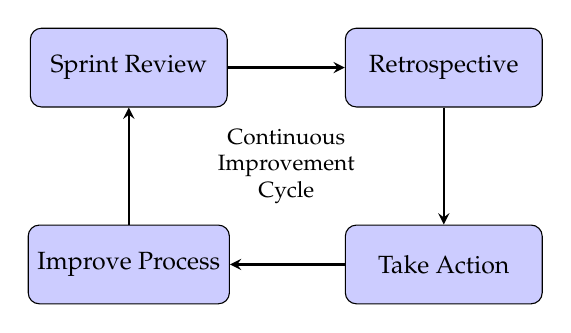
\begin{tikzpicture}
    % Define styles
    \tikzstyle{process} = [rectangle, rounded corners, minimum width=2.5cm, minimum height=1cm,
                          text centered, draw=black, fill=blue!20, font=\small]
    \tikzstyle{arrow} = [thick,->,>=stealth]

    % Nodes positioned absolutely
    \node[process] (review) at (0,0) {Sprint Review};
    \node[process] (retro) at (4,0) {Retrospective};
    \node[process] (action) at (4,-2.5) {Take Action};
    \node[process] (improve) at (0,-2.5) {Improve Process};

    % Arrows
    \draw[arrow] (review) -- (retro);
    \draw[arrow] (retro) -- (action);
    \draw[arrow] (action) -- (improve);
    \draw[arrow] (improve) -- (review);

    % Center label
    \node[font=\footnotesize, text width=2cm, align=center] at (2,-1.25) {Continuous\\Improvement\\Cycle};
\end{tikzpicture}
\caption{Continuous improvement cycle through regular sprint reviews and retrospectives}
\label{fig:improvement-cycle}
\end{figure}


The combination of sprint reviews, retrospectives, and lightweight metrics creates continuous improvement. The organization demonstrates that Agile evaluation doesn't require sophisticated tools or extensive data collection. Regular inspection of both product and process, coupled with willingness to adapt when issues surface, drives meaningful improvement over time.

Management support reinforces this learning orientation \textbf{(Transcript: 00:24:22--00:25:22)}, allowing them to invest time in addressing problems rather than only delivering features. Leadership provides resources for skill development and respects process boundaries. When they request tools or training, management evaluates requests seriously. This support creates psychological safety where teams can acknowledge problems without fear, enabling honest retrospectives and genuine improvement.

\chapter{Understanding Stakeholder Voices}
\label{ch:stakeholder-mapping}

Successful Agile implementation depends on understanding and engaging stakeholders effectively. Research with 2,000 Scrum teams found that stakeholder concern is a key driver of team effectiveness \textit{\parencite{verwijs2021scrum}}. Djøf Trade Union gradually learned to identify stakeholders and build collaborative relationships that support value delivery.

\section{Stakeholder Identification and Collaboration}
\label{sec:identifying-stakeholders}

The organization serves two groups: internal employees and union members. Internal employees use systems for booking management and account administration \textbf{(Transcript: 00:01:34--00:02:04)}. Union members interact with member-facing systems. These two stakeholder groups create challenges because internal and member needs don't always align.

The Product Owner became the bridge between stakeholder groups and the development team. Before Scrum, tasks arrived chaotically without clear understanding of who needed the work or why. The Product Owner now gathers needs from both groups, translates them into backlog items, and ensures the team understands context \textbf{(Transcript: 00:11:22--00:11:52)}.

They recognized that stakeholders have different influence and interest levels. Leadership cares about member growth and operational efficiency. They set budget priorities and decide which initiatives receive funding. Daily system users provide practical feedback about what works and what frustrates them.

% Figure: Stakeholder Landscape
% Simple narrative showing two stakeholder groups and Product Owner bridge

\begin{figure}[htbp]
    \centering
    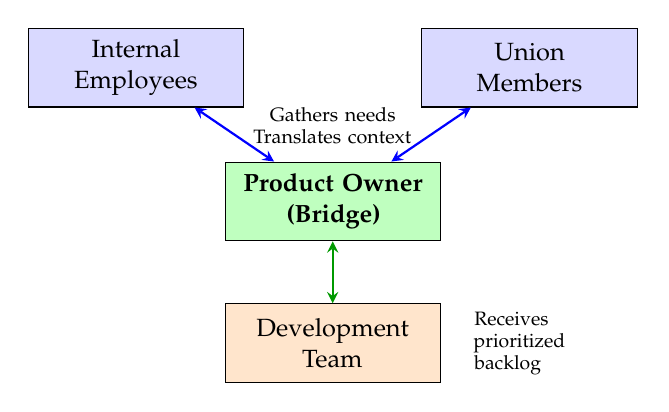
\begin{tikzpicture}[
        stakeholder/.style={rectangle, draw, fill=blue!15, text width=2.5cm, align=center, minimum height=1cm, font=\small},
        po/.style={rectangle, draw, fill=green!25, text width=2.5cm, align=center, minimum height=1cm, font=\small\bfseries},
        team/.style={rectangle, draw, fill=orange!20, text width=2.5cm, align=center, minimum height=1cm, font=\small},
        arrow/.style={<->, >=stealth, thick}
    ]

    % Top section - Stakeholder groups
    \node[stakeholder] (internal) at (0,3.5) {Internal\\Employees};
    \node[stakeholder] (members) at (5,3.5) {Union\\Members};

    % Middle - Product Owner (the bridge)
    \node[po] (po) at (2.5,1.8) {Product Owner\\(Bridge)};

    % Bottom - Development Team
    \node[team] (team) at (2.5,0) {Development\\Team};

    % Arrows showing flow
    \draw[arrow, blue] (internal) -- (po);
    \draw[arrow, blue] (members) -- (po);
    \draw[arrow, green!60!black] (po) -- (team);

    % Labels
    \node[above=0.1cm of po, font=\scriptsize, text width=2cm, align=center] {Gathers needs\\Translates context};
    \node[right=0.3cm of team, font=\scriptsize, text width=2cm, align=left] {Receives\\prioritized\\backlog};

    \end{tikzpicture}
    \caption{Stakeholder landscape showing two groups served by Ahmed's organization. The Product Owner bridges stakeholder groups and the development team, gathering needs from both internal employees and union members, then translating them into prioritized backlog items.}
    \label{fig:jawad-stakeholder-landscape}
\end{figure}


Refinement created opportunities for stakeholders to shape solutions before development begins. The team now breaks down epics collaboratively with input from users \textbf{(Transcript: 00:05:30--00:06:00)}. When stakeholders participate in defining acceptance criteria, they gain realistic expectations.

Sprint reviews became regular touchpoints where stakeholders see completed work and provide feedback. The team invites business representatives to reviews, demonstrating features and gathering reactions \textbf{(Transcript: 00:20:37--00:21:07)}. Quarterly demos expanded this transparency by showcasing three months of progress to broader audiences.

Direct stakeholder-to-developer communication still happens. Ahmed adapted practically: when users approach him with ideas, he listens but redirects them to the Product Owner for prioritization \textbf{(Transcript: 00:29:22--00:30:21)}. This protects the team while recognizing valuable ideas.

\section{Managing Competing Interests and Communication}
\label{sec:competing-interests}

Stakeholders do not always agree. Economic constraints take priority: when leadership determines something costs too much, the project stops regardless of user enthusiasm \textbf{(Transcript: 00:36:17--00:36:47)}. Technical feasibility also matters. When requests would compromise system integrity, developers push back with Product Owner support.

The team learned to find middle ground. Understanding underlying needs often reveals alternative solutions. Successful Agile transformations require balancing multiple influences, with developer skills and management support being critical factors \textit{\parencite{russo2021agile}}.

Stakeholder management improved significantly with Agile practices. Structured refinement, regular reviews, transparent backlog, and clear Product Owner ownership created predictability that reduces frustration. Stakeholders know when to expect features. Management sees progress through transparent metrics rather than status reports that may hide problems.

The team established multiple feedback channels tailored to different stakeholder groups. Members receive newsletters announcing new features and changes, creating awareness without direct development team involvement. Internal stakeholders participate in sprint reviews and can observe the Jira backlog. Leadership receives quarterly progress updates aligned with strategic objectives. These layered communication approaches ensure each stakeholder group receives appropriate information without overwhelming the development team with coordination demands.

\chapter{Software Quality and Technology Integration}
\label{ch:software-quality}

\section{Quality Management}
\label{sec:quality-management}

% Your content here


\section{Technology Opportunities}
\label{sec:technology-opportunities}

% Your content here


\section{Tools and Practices}
\label{sec:tools-practices}

% Your content here

\chapter{Deployment Practices and System Observability}
\label{ch:production-pipeline}

Djøf Trade Union's deployment pipeline functions reliably but reveals opportunities for improvement. They manually approve each deployment stage, tests sometimes fail unpredictably, and monitoring gaps delay problem detection \textbf{(Transcript: 00:37:52)}.

\section{Current Pipeline and Monitoring Assessment}
\label{sec:current-pipeline}

Their current pipeline moves code through dev, test, and production environments \textbf{(Transcript: 00:31:37--00:32:07)}. Automated builds run unit tests, integration tests, and static analysis. However, deployment requires manual approval at each stage \textbf{(Transcript: 00:34:07--00:34:37)}.

Tests occasionally fail without reason and require reruns \textbf{(Transcript: 00:37:52)}. This instability wastes developer time and erodes confidence in test results. When tests fail randomly, they can't distinguish real problems from false alarms.

% Figure: Pipeline Current vs Recommended State
% Comparison of deployment pipeline practices

\begin{figure}[htbp]
    \centering
    \resizebox{0.9\textwidth}{!}{%
    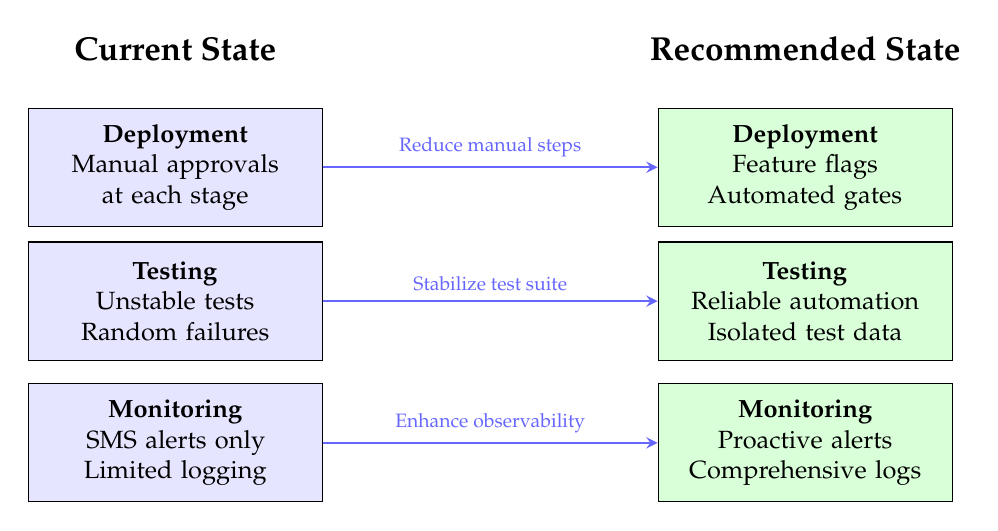
\begin{tikzpicture}[
        box/.style={rectangle, draw, fill=blue!10, text width=3.5cm, align=center, minimum height=1.5cm, font=\small},
        goodbox/.style={rectangle, draw, fill=green!15, text width=3.5cm, align=center, minimum height=1.5cm, font=\small},
        title/.style={font=\bfseries\large},
        arrow/.style={->, >=stealth, thick}
    ]

    % Current State (Left)
    \node[title] (current) at (0,5) {Current State};

    \node[box] (c1) at (0,3.5) {\textbf{Deployment}\\Manual approvals\\at each stage};
    \node[box] (c2) at (0,1.8) {\textbf{Testing}\\Unstable tests\\Random failures};
    \node[box] (c3) at (0,0) {\textbf{Monitoring}\\SMS alerts only\\Limited logging};

    % Recommended State (Right)
    \node[title] (recommended) at (8,5) {Recommended State};

    \node[goodbox] (r1) at (8,3.5) {\textbf{Deployment}\\Feature flags\\Automated gates};
    \node[goodbox] (r2) at (8,1.8) {\textbf{Testing}\\Reliable automation\\Isolated test data};
    \node[goodbox] (r3) at (8,0) {\textbf{Monitoring}\\Proactive alerts\\Comprehensive logs};

    % Connecting arrows with improvement labels
    \draw[arrow, blue!60] (c1) -- node[above, font=\scriptsize] {Reduce manual steps} (r1);
    \draw[arrow, blue!60] (c2) -- node[above, font=\scriptsize] {Stabilize test suite} (r2);
    \draw[arrow, blue!60] (c3) -- node[above, font=\scriptsize] {Enhance observability} (r3);

    \end{tikzpicture}%
    }
    \caption{Comparison of current and recommended pipeline practices. Current state relies on manual approvals and reactive monitoring. Recommended improvements focus on automation, test stability, and comprehensive observability to enable faster feedback and reduce operational overhead.}
    \label{fig:jawad-pipeline-comparison}
\end{figure}


Monitoring relies on SMS alerts for critical failures \textbf{(Transcript: 00:36:37)}. If problems occur overnight, the team discovers them the next morning. Limited logging makes root cause analysis difficult \textbf{(Transcript: 00:37:52--00:38:22)}.

The most impactful improvement would be comprehensive logging and monitoring \textbf{(Transcript: 00:38:37)}. Detailed logs capture system behavior. Proactive alerts detect anomalies before they escalate. This reduces response time and prevents user impact.

\section{Test Stability Improvements}
\label{sec:test-stability}

Stabilizing tests eliminates false failures. Isolating test data, managing test dependencies, and identifying flaky tests creates reliable automation. When teams trust their tests, they deploy confidently.

Gradually reducing manual approvals accelerates deployment. Feature flags enable safe production releases without manual gates. Teams can toggle features independently from deployment.

\section{Building Deployment Capabilities}
\label{sec:deployment-capabilities}

Enhanced observability transforms operations. Distributed tracing reveals request flows across services. Centralized logging aggregates data for analysis. Custom dashboards surface critical metrics in real time.

Improving deployment frequency builds organizational capability. More frequent deployments reduce batch size, making problems easier to diagnose and fixes faster to deploy.

Investing in test infrastructure pays dividends. Container-based test environments ensure consistency. Parallel test execution reduces feedback time. Regular test suite maintenance removes obsolete tests.

\chapter{Conclusion}
\label{ch:conclusion}

Djøf Trade Union transformed chaotic development practices into structured, predictable delivery through pragmatic Scrum adoption. Their journey from ad-hoc task assignment to refined backlog management illustrates how Agile frameworks address fundamental organizational impediments when adapted thoughtfully to context.

The failed membership checkbox project crystallized the costs of absent process controls. Two weeks of development investment vanished because no gatekeeping process verified legal compliance or vendor capability before work began. This painful lesson catalyzed the adoption of refinement sessions that now surface blockers proactively. Their refinement practice demonstrates that breaking down epics collaboratively with clear acceptance criteria prevents wasted effort and aligns stakeholder expectations.

Their flexibility in adapting Scrum reveals maturity beyond rigid framework adherence. Dropping story points when stakeholders misunderstood them and occasionally skipping retrospectives when sprints lacked meaningful progress shows they value outcomes over ceremony. This pragmatism reflects understanding that frameworks serve teams rather than constrain them.

\section{Emerging Challenges}
\label{sec:emerging-challenges}

Legacy system complexity and test instability represent ongoing impediments. Flaky tests that fail randomly erode confidence and waste developer time. Limited monitoring visibility delays problem detection, particularly for overnight failures. These technical gaps suggest areas for continued investment.

\section{Future Development}
\label{sec:future-development}

The organization built strong foundations through refinement discipline, role clarity, and stakeholder collaboration. Enhancing observability, stabilizing test automation, and gradually reducing manual deployment gates will extend their Agile maturity. Their demonstrated willingness to adapt practices positions them well for continued evolution.


% ============================================================================
% BIBLIOGRAPHY
% ============================================================================
\cleardoublepage
\phantomsection
% Include all bibliography entries even if not cited
\nocite{*}
\printbibliography[heading=bibintoc,title={Bibliography}]

% ============================================================================
% APPENDIX
% ============================================================================
\cleardoublepage
\appendix
\chapter{Interview Questions}
\label{app:interview-questions}

\section{Introduction}
\label{app:introduction}

\begin{enumerate}
    \item Can you briefly introduce yourself and your role within the company?
    \item How does your role specifically influence Agile practices or project outcomes?
    \item What was the organization's key motivation for transitioning to Agile?
    \item What specific Agile frameworks are being used to manage pipeline processes?
    \item How has top management supported Agile adoption or Agile practices?
\end{enumerate}

\section{Project Success and Failure Factors}
\label{app:success-factors}

\begin{enumerate}
    \item What critical factors contribute to the success of your software projects?
    \item Are there any successful projects you can share, or any unexpected outcomes?
    \item How do success factors vary across different types of projects?
    \item What lessons from failed projects were applied to improve Agile practices?
    \item How do you ensure continuous improvement and avoid complacency?
\end{enumerate}

\section{Professional Role Alignment}
\label{app:role-alignment}

\begin{enumerate}
    \item How do Product Owners ensure alignment with end-user needs?
    \item How do Scrum Masters manage conflicts or impediments during development?
    \item How do leadership roles influence alignment within your team?
    \item How do developers contribute to maintaining alignment?
    \item How do you maintain alignment during high-pressure scenarios?
\end{enumerate}

\section{Development Process Discussion}
\label{app:development-process}

\begin{enumerate}
    \item Can you describe your development process and methodologies used?
    \item What motivated your organization to adopt this methodology?
    \item How does your methodology support rapid iterations or quick pivots?
\end{enumerate}

\section{Monitoring and Improvement Strategies}
\label{app:monitoring}

\begin{enumerate}
    \item How do you measure team effectiveness and project success?
    \item What strategies do you use for continuous improvement?
    \item How do feedback loops influence prioritization of improvement areas?
    \item What training or support mechanisms enhance developers' skills?
    \item How do tools like dashboards or AI-based insights help improve performance?
    \item What long-term metrics do you monitor for sustained success?
\end{enumerate}

\section{Software Pipeline}
\label{app:pipeline}

\begin{enumerate}
    \item What tools or platforms do you use to automate your pipeline?
    \item How do you measure the reliability and efficiency of your pipeline?
    \item What are the most common challenges when maintaining or scaling the pipeline?
    \item Can you share a specific example of a major issue and how it was resolved?
    \item Are any future advancements or technologies considered to enhance the pipeline?
\end{enumerate}

\section{Generative AI in the Software Pipeline}
\label{app:generative-ai}

\begin{enumerate}
    \item Has your company integrated Generative AI into its software development pipeline?
    \item What has been the impact on productivity, quality, and team dynamics?
    \item What challenges or limitations have you encountered when using Generative AI tools?
    \item How has Generative AI influenced your ability to meet customer needs?
    \item What was the process of adopting Generative AI tools?
    \item How does Generative AI integrate with your Agile development practices?
\end{enumerate}

\section{Summary and Feedback}
\label{app:summary}

\begin{enumerate}
    \item Is there anything we haven't discussed that you believe is critical?
    \item What trends in Agile do you think will shape its future implementation?
    \item What emerging technologies or methodologies do you foresee influencing Agile practices?
\end{enumerate}


\end{document}